\documentclass[a4paper,14pt]{extarticle}
\usepackage{geometry}

\usepackage{cmap} % Улучшенный поиск русских слов в полученном pdf-файле
\usepackage{mathtext} % русские буквы в формулах
\defaulthyphenchar=127 % Если стоит до fontenc, то переносы не впишутся в выделяемый текст при копировании его в буфер обмена
\usepackage[T2A]{fontenc} % кодировка
\usepackage[utf8]{inputenc}
\usepackage[english, russian]{babel}
\usepackage{pscyr}
\renewcommand{\rmdefault}{ftm} % ftm - (TimesNewRoman), fac - Academy, fad - Advertisement, flz - Lazurski, fcr - CourierNewPSM, others in pscyr.sty

\usepackage{amsthm,amsfonts,amsmath,amssymb,amscd} % Математические дополнения от AMS
\usepackage{mathtools} % Добавляет окружение multlined

\usepackage{longtable} % Длинные таблицы
\usepackage{multirow,makecell,array} % Улучшенное форматирование таблиц
\usepackage{booktabs} % Возможность оформления таблиц в классическом книжном стиле (при правильном использовании не противоречит ГОСТ)

\usepackage{soulutf8} % Поддержка переносоустойчивых подчёркиваний и зачёркиваний
\usepackage{icomma} % Запятая в десятичных дробях

\usepackage[usenames,dvipsnames,svgnames,table,rgb]{xcolor}

\usepackage{hyperref}

\usepackage{graphicx} % Подключаем пакет работы с графикой
\graphicspath{{../images/}{images/}} % Пути к изображениям

%%% Подписи %%%
\usepackage[singlelinecheck=off,center]{caption}
\usepackage{subcaption}
\usepackage[onehalfspacing]{setspace}

%%% Списки %%%
\usepackage{enumitem}

%%% Библиография %%%
\usepackage{cite}                                   % Красивые ссылки на литературу

%%% Оглавление %%%
\usepackage[nottoc]{tocbibind}
\usepackage{tocloft}
\usepackage{titlesec}

\geometry{a4paper,top=2cm,bottom=2cm,left=2cm,right=1cm}
%%% Выравнивание и переносы %%%
\sloppy                             % Избавляемся от переполнений
\clubpenalty=10000                  % Запрещаем разрыв страницы после первой строки абзаца
\widowpenalty=10000                 % Запрещаем разрыв страницы после последней строки абзаца
\usepackage{indentfirst}
\frenchspacing
\setlength{\parindent}{2.5em} % Абзацный отступ
\linespread{1.3}

% colors
\definecolor{linkcolor}{rgb}{0.9,0,0}
\definecolor{citecolor}{rgb}{0,0.6,0}
\definecolor{urlcolor}{rgb}{0,0,1}
\definecolor{mygreen}{rgb}{0,0.6,0}
\definecolor{mygray}{rgb}{0.5,0.5,0.5}
\definecolor{mymauve}{rgb}{0.58,0,0.82}

\hypersetup{				% Гиперссылки
    unicode=true,          % non-Latin characters in Acrobat’s bookmarks
    pdftoolbar=true,        % show Acrobat’s toolbar?
    pdfmenubar=true,        % show Acrobat’s menu?
    pdffitwindow=false,     % window fit to page when opened
    pdfstartview={FitH},    % fits the width of the page to the window
    pdftitle={Применение глубоких свёрточных нейронных сетей для решения задачи распознавания образов},    % title
    pdfauthor={Юткин Дмитрий Игоревич},     % author
    pdfsubject={Курсовая},   % subject of the document
    pdfcreator={Юткин Дмитрий Игоревич},   % creator of the document
    pdfproducer={Юткин Дмитрий Игоревич}, % producer of the document
    pdfkeywords={convolutional} {neural} {networks} 
    {deeplearning} {deep} {learning} {caffe} {сверточные} {нейронные} {сети}
    {глубокое} {обучение} {компьютерное} {зрение}, % Ключевые слова
    pdfnewwindow=true,
    pdflang={ru},
    linktocpage=true,
    plainpages=false,
    colorlinks,       	    % false: ссылки в рамках; true: цветные ссылки
    linkcolor={linkcolor},      % цвет ссылок типа ref, eqref и подобных
    citecolor={citecolor},      % цвет ссылок-цитат
    urlcolor={urlcolor},        % цвет гиперссылок
}

%% Рисунки %%%
\DeclareCaptionLabelSeparator{emdash}{~--- }
\captionsetup[figure]{labelsep=emdash,font=onehalfspacing,position=bottom}
\captionsetup{%
    singlelinecheck=off,                % Многострочные подписи, например у таблиц
    skip=2pt,                           % Вертикальная отбивка между подписью и содержимым рисунка или таблицы определяется ключом
    justification=centering,            % Центрирование подписей, заданных командой \caption
}

%% Подписи подрисунков %%%
\renewcommand{\thesubfigure}{\asbuk{subfigure}}           % Буквенные номера подрисунков
\captionsetup[subfigure]{font={normalsize},               % Шрифт подписи названий подрисунков (не отличается от основного)
    labelformat=brace,                                    % Формат обозначения подрисунка
    justification=centering,                              % Выключка подписей (форматирование), один из вариантов            
}

%%% Списки %%%
% Используем короткое тире (endash) для ненумерованных списков (ГОСТ 2.105-95, пункт 4.1.7, требует дефиса, но так лучше смотрится)
\renewcommand{\labelitemi}{\normalfont\bfseries{--}}

% Перечисление строчными буквами русского алфавита (ГОСТ 2.105-95, 4.1.7)
\makeatletter
    \AddEnumerateCounter{\asbuk}{\russian@alph}{щ}
\makeatother
\setlist[enumerate,1]{label=\asbuk{enumi})} % первого уровня 1), 2)...
\setlist[enumerate,2]{label=\arabic*)} % второго уровня а), б) ... 

\setlist{nosep,%                                    % Единый стиль для всех списков (пакет enumitem), без дополнительных интервалов.
    labelindent=\parindent,leftmargin=*%            % Каждый пункт, подпункт и перечисление записывают с абзацного отступа
}

%%% Переопределение именований %%%
\addto\captionsrussian{%
    \renewcommand{\partname}{Часть}
    \renewcommand{\abstractname}{Аннотация}
    \renewcommand{\contentsname}{Оглавление} % (ГОСТ Р 7.0.11-2011, 4)
    \renewcommand{\figurename}{Рисунок} % (ГОСТ Р 7.0.11-2011, 5.3.9)
    \renewcommand{\tablename}{Таблица} % (ГОСТ Р 7.0.11-2011, 5.3.10)
    \renewcommand{\indexname}{Предметный указатель}
    \renewcommand{\listfigurename}{Список рисунков}
    \renewcommand{\listtablename}{Список таблиц}
}
%
%%% Старт отсчет страниц с титульника
\makeatletter
\renewenvironment{titlepage}
 {%
  \if@twocolumn
    \@restonecoltrue\onecolumn
  \else
    \@restonecolfalse\newpage
  \fi
  \thispagestyle{empty}%
 }
 {%
  \if@restonecol
    \twocolumn
  \else
    \newpage
  \fi
 }
\makeatother
%%%

%%% Библиография %%%
\makeatletter
\bibliographystyle{utf8gost71u}     % Оформляем библиографию по ГОСТ 7.1 (ГОСТ Р 7.0.11-2011, 5.6.7)
\renewcommand{\@biblabel}[1]{#1.}   % Заменяем библиографию с квадратных скобок на точку
\makeatother

%%% Оглавление %%%
\cftsetrmarg{2.55em plus1fil} %To have the (sectional) titles in the ToC, etc., typeset ragged right with no hyphenation
\renewcommand{\cftsecdotsep}{\cftdotsep} % отбивка точками до номера страницы начала главы/раздела
\renewcommand{\cftsecpagefont}{\normalfont}        % нежирные номера страниц у глав в оглавлении
\renewcommand{\cftsecleader}{\cftdotfill{\cftsecdotsep}}% нежирные точки до номеров страниц у глав в оглавлении
\renewcommand{\cfttoctitlefont}{\filright\fontsize{16pt}{18pt}\selectfont\bfseries} % Размер заголовка оглавления

%\renewcommand{\cftsecfont}{}                       % нежирные названия глав в оглавлении
%\renewcommand\cftsecaftersnum{.\ }   % добавляет точку с пробелом после номера раздела в оглавлении
%\renewcommand\cftsecaftersnum{.\ }    % добавляет точку с пробелом после номера подраздела в оглавлении
%\renewcommand\cftsubsecaftersnum{.\ } % добавляет точку с пробелом после номера подподраздела в оглавлении
%\renewcommand\cftsecaftersnum{\quad}     % добавляет \quad после номера раздела в оглавлении
%\renewcommand\cftsecaftersnum{\quad}      % добавляет \quad после номера подраздела в оглавлении
%\renewcommand\cftsubsecaftersnum{\quad}   % добавляет \quad после номера подподраздела в оглавлении
%\addtocontents{toc}{~\hfill{Стр.}\par}% добавить Стр. над номерами страниц

%%% Оформление заголовков глав, разделов, подразделов %%%
\titleformat{\section}[block]
    %{\filcenter\fontsize{16pt}{18pt}\selectfont\bfseries}{\thesection\cftsecaftersnum}{0.5em}{} % по центру
    {\filright\fontsize{16pt}{18pt}\selectfont\bfseries}{\thesection\cftsecaftersnum}{0.5em}{} % справа

\titleformat{\subsection}[block]
    %{\filcenter\fontsize{16pt}{18pt}\selectfont\bfseries}{\thesubsection\cftsubsecaftersnum}{0.5em}{}
    {\filright\fontsize{16pt}{18pt}\selectfont\bfseries}{\thesubsection\cftsubsecaftersnum}{0.5em}{}

\titleformat{\subsubsection}[block]
    %{\filcenter\fontsize{16pt}{18pt}\selectfont\bfseries}{\thesubsubsection\cftsubsecaftersnum}{0.5em}{}
    {\filright\fontsize{16pt}{18pt}\selectfont\bfseries}{\thesubsubsection\cftsubsecaftersnum}{0.5em}{}

%\renewcommand{\abstractnamefont}{\fontsize{16pt}{18pt}\selectfont\bfseries} % Размер заголовка аннтоации


% Расстояние между текстом и заголовками
%\setlength{\abstitleskip}{-25pt} % расстояние между заголовком аннтоации и тестом
\titlespacing{\section}{\parindent}{*2}{*1} % Расстояние между заголовком раздела и текстом должно быть равно удвоенному межстрочному интервалу.  Расстояние между основаниями строк заголовка принимают такими же, как в тексте
\titlespacing{\subsection}{\parindent}{*2}{*1}
\titlespacing{\subsubsection}{\parindent}{*2}{*1}

% Listings
\lstset{ %
  backgroundcolor=\color{white},   % choose the background color; you must add \usepackage{color} or \usepackage{xcolor}
  basicstyle=\ttfamily\footnotesize,        % the size of the fonts that are used for the code
  breakatwhitespace=false,         % sets if automatic breaks should only happen at whitespace
  breaklines=true,                 % sets automatic line breaking
  captionpos=b,                    % sets the caption-position to bottom
  commentstyle=\ttfamily,    % comment style
  columns=fixed,
  deletekeywords={...},            % if you want to delete keywords from the given language
  escapeinside={\%*}{*)},          % if you want to add LaTeX within your code
  extendedchars=true,              % lets you use non-ASCII characters; for 8-bits encodings only, does not work with UTF-8
  frame=none,	                   % adds a frame around the code
  keepspaces=true,                 % keeps spaces in text, useful for keeping indentation of code (possibly needs columns=flexible)
  keywordstyle=\ttfamily\bfseries,       % keyword style
  otherkeywords={*,...},           % if you want to add more keywords to the set
  numbers=left,                    % where to put the line-numbers; possible values are (none, left, right)
  numbersep=5pt,                   % how far the line-numbers are from the code
  numberstyle=\footnotesize\color{mygray}, % the style that is used for the line-numbers
  rulecolor=\color{black},         % if not set, the frame-color may be changed on line-breaks within not-black text (e.g. comments (green here))
  showspaces=false,                % show spaces everywhere adding particular underscores; it overrides 'showstringspaces'
  showstringspaces=false,          % underline spaces within strings only
  showtabs=false,                  % show tabs within strings adding particular underscores
  stepnumber=1,                    % the step between two line-numbers. If it's 1, each line will be numbered
  stringstyle=\ttfamily,     % string literal style
  tabsize=4,	                   % sets default tabsize to 2 spaces
  title=\lstname                   % show the filename of files included with \lstinputlisting; also try caption instead of title
  % stringstyle=\color{mymauve}\ttfamily,     % string literal style
  % keywordstyle=\ttfamily\color{blue},       % keyword style
  % commentstyle=\ttfamily\color{mygreen},    % comment style
} % Файл с настройкой стилей


\begin{document}
\begin{titlepage}
    \begin{center}
        ФЕДЕРАЛЬНОЕ ГОСУДАРСТВЕННОЕ АВТОНОМНОЕ
        
        ОБРАЗОВАТЕЛЬНОЕ УЧРЕЖДЕНИЕ
        
        ВЫСШЕГО ОБРАЗОВАНИЯ
        
       <<НАЦИОНАЛЬНЫЙ ИССЛЕДОВАТЕЛЬСКИЙ УНИВЕРСИТЕТ
       
       ''ВЫСШАЯ~ШКОЛА~ЭКОНОМИКИ''>>
       \vspace{1cm}
 
        \textbf{Московский институт электроники и математики}
        
        Юткин Дмитрий Игоревич, группа БИВ-141
        \vspace{1cm}
        
        \textbf{\MakeUppercase{Применение глубоких свёрточных нейронных сетей для решения задачи распознавания образов}}
        \vspace{1cm}

        Междисциплинарная курсовая работа
        
        по направлению 09.03.01.62 Информатика и вычислительная техника 

        студента образовательной программы бакалавриата
        
        <<Информатика и вычислительная техника>>
        
    \end{center}
    \begin{flushright}
        Студент~\rule{4cm}{.1pt}~Д.И.\,Юткин
        \vspace{1cm}
        
        Научный руководитель

        Старший преподаватель

        Д.В.\,Пантюхин
        
        \rule{4cm}{.1pt}
    \end{flushright}
    \vfill\center{Москва 2016 г.}
\end{titlepage} % Титульник
\section*{Аннотация}
Работа посвящена решению задачи распознавания образов с использованием глубоких свёрточных 
нейронных сетей. В результате исследования было обучено несколько нейронных сетей различной глубины 
(от 9 до 18 слоёв), часть из которых обучалась на предварительно обработанных данных. Максимальная 
точность одиночной модели составила 93,4\%, объединение нейронных сетей в ансамбль позволило
увеличилась точность распознавания до 94,21\%, что сравнимо с точностью человека. Все эксперименты 
проводились на наборе изображений CIFAR-10, с использованием графических процессоров и фреймворка
для глубокого обучения Caffe.

\section*{Abstract}
The research focused on application of deep convolutional neural networks for
solving object recognition task in natural images. As a result, several models of different depth
(from 9 to 18 layers) have been trained on preprocessed and augmented data. The best model has shown accuracy 
of 93,4\% on a test images. Whereas, ensemble of combined models has achived 94,21\% which is 
close-to-human performance. All experiments have been carried out on the CIFAR-10 dataset with modern GPUs
and Caffe framework for a deep learning. % Аннотация

\tableofcontents
\clearpage

\section{Введение}
Идейные соображения высшего порядка, а \textbf{также} рамки и место обучения кадров обеспечивает широкому кругу (специалистов) участие в формировании позиций, занимаемых участниками в отношении поставленных задач. С другой стороны реализация намеченных плановых заданий играет важную роль в формировании форм развития. 

\begin{figure}[h]
    \centering
    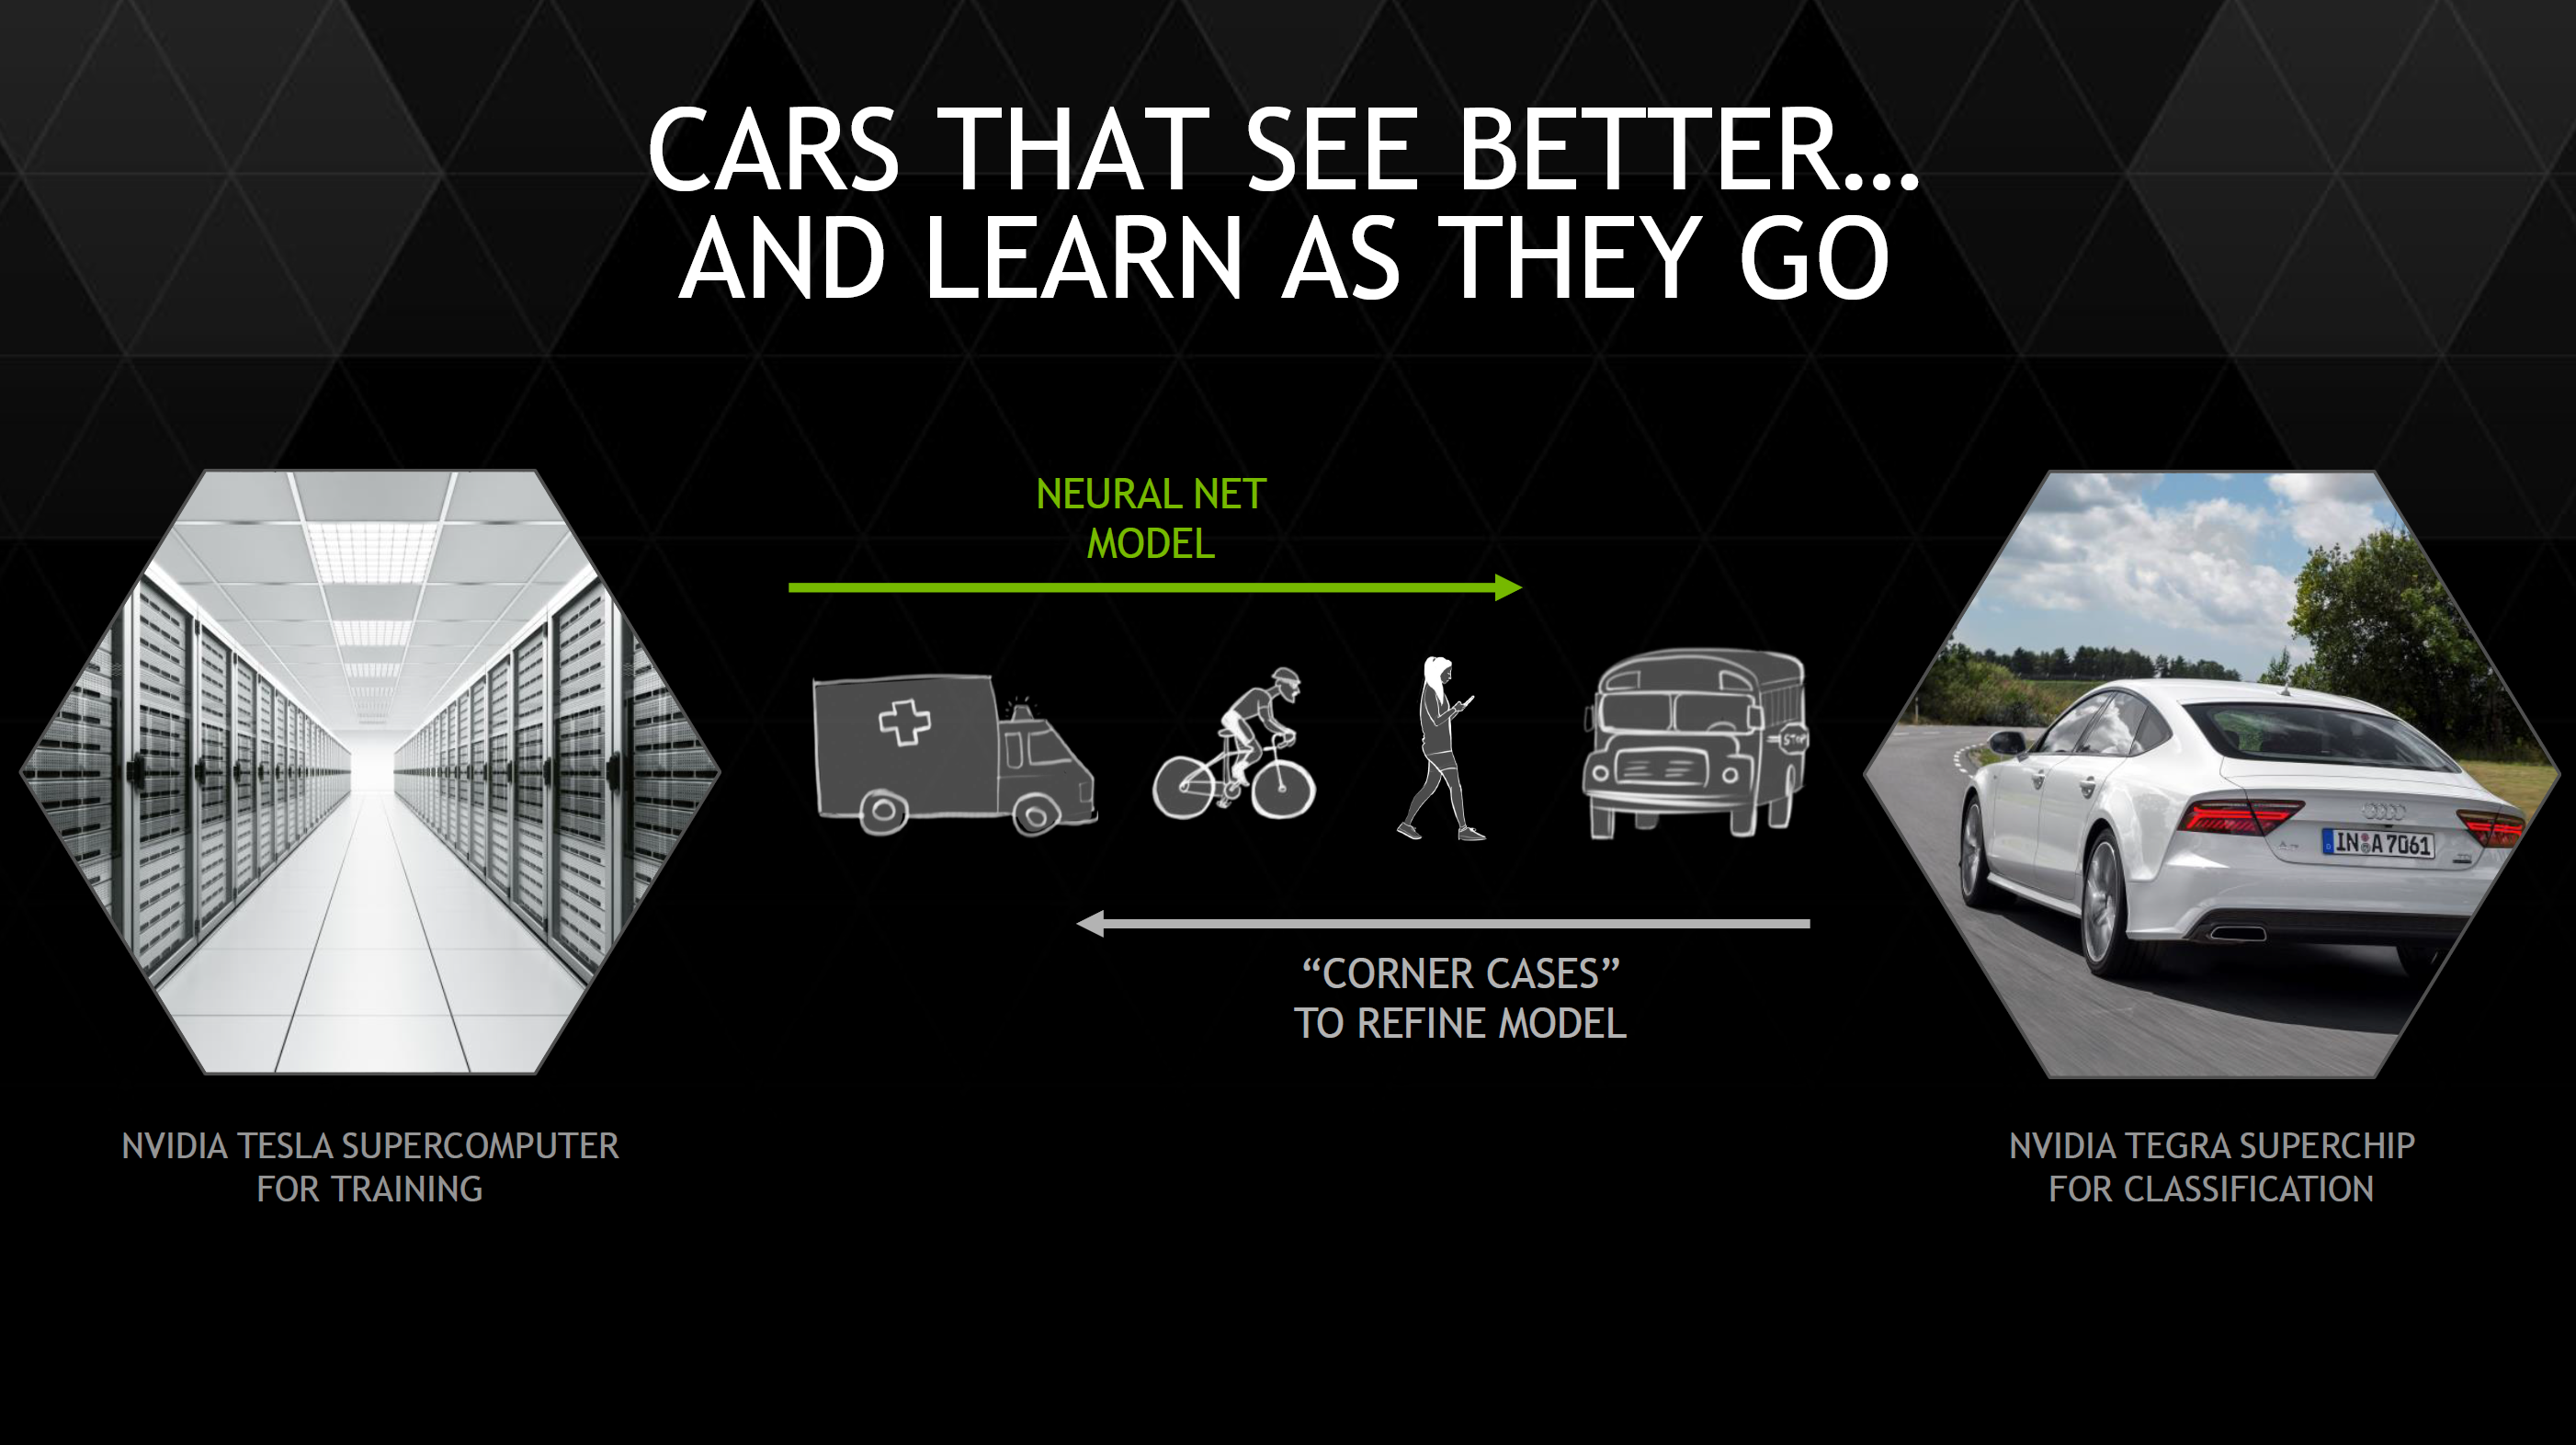
\includegraphics[width=0.8\textwidth]{test.png}
    \caption{Прекрасная подпись к рисунку}
\end{figure}

Повседневная практика показывает, что начало повседневной работы по формированию позиции позволяет выполнять важные задания по разработке форм развития. Таким образом консультация с широким активом обеспечивает широкому кругу (специалистов) участие в формировании дальнейших направлений развития.
\begin{enumerate}
\item The first item
    \begin{enumerate}
    \item Nested item 1
    \item Nested item 2
    \end{enumerate}
\item The second item
\item The third etc \ldots
\end{enumerate}

\begin{itemize}
\item more work
\item more responsibility
\item more satisfaction
\end{itemize}

\subsection{Sub-section}
Значимость этих проблем настолько очевидна, что начало повседневной работы по формированию позиции представляет собой интересный эксперимент проверки модели развития. Значимость этих проблем настолько очевидна, что начало повседневной работы по формированию позиции играет важную роль в формировании существенных финансовых и административных условий. Товарищи! консультация с широким активом обеспечивает широкому кругу (специалистов) участие в формировании новых предложений. Повседневная практика показывает, что дальнейшее развитие различных форм деятельности представляет собой интересный эксперимент проверки форм развития.
\subsubsection{Sub-sub-section}
Значимость этих проблем настолько очевидна, что начало повседневной работы по формированию позиции представляет собой интересный эксперимент проверки модели развития. Значимость этих проблем настолько очевидна, что начало повседневной работы по формированию позиции играет важную роль в формировании существенных финансовых и административных условий. Товарищи! консультация с широким активом обеспечивает широкому кругу (специалистов) участие в формировании новых предложений. Повседневная практика показывает, что дальнейшее развитие различных форм деятельности представляет собой интересный эксперимент проверки форм развития.
\section{Еще Текст}
Blablabla said Nobody ~\cite{einstein}. to you how all this mistaken idea of denouncing pleasure and praising pain was born and I will give you a complete account of the system, and expound the actual teachings of the great explorer of the truth, the master-builder of human happiness. No one rejects, dislikes, or avoids pleasure itself, because it is pleasure, but because those who do not know how to pursue pleasure rationally encounter consequences that are extremely painful. Nor again is there anyone who loves or pursues or desires to obtain pain of itself, because it is pain, but because occasionally circumstances occur in which toil and pain can procure him some great pleasure. To take a trivial example, which of us ever undertakes laborious physical exercise, except to obtain some advantage from it? But who has any right to find fault with a man who chooses to enjoy a pleasure that has no annoying consequences, or one who avoids a pain that produces no resultant pleasure?"

\clearpage
\bibliography{biblio}
\end{document}